\section{Ruport}

\begin{itemize}
\item Documentación de la API: \htmladdnormallink{http://api.rubyreports.org/}{http://api.rubyreports.org/}
\item Ejemplos: \htmladdnormallink{http://www.rubyreports.org/examples.html}{http://www.rubyreports.org/examples.html}
\end{itemize}

\begin{verbatim}
~/rubytesting/TheRubyProgrammingLanguage/chapter8ReflectionandMetaprogramming$ cat -n ruport_example.rb 
     1  require 'ruport'
     2  
     3  table = Ruport::Data::Table.new(
     4     :column_names => [               "alu",      "nota"],
     5     :data         => [ 
     6                        ["Almeida Gonzalez",         4.5],
     7                        ["Hernandez Perez",          6.5],
     8                        ["Mendez Chavez",            4.5],
     9                        ["Rodriguez Luis",           9.5]
    10                      ]
    11  )
    12  
    13  puts table.to_text
    14  
    15  dubious = table.rows_with_nota(4.5)
    16  dubious.each do |cal|
    17    puts cal.to_csv
    18  end

\end{verbatim}

\begin{verbatim}
~$ sudo gem install ruport
Password:
Fetching: fastercsv-1.5.4.gem (100%)
Fetching: color-1.4.1.gem (100%)
Fetching: hoe-2.12.3.gem (100%)
Fetching: transaction-simple-1.4.0.gem (100%)
WARNING: transaction-simple-1.4.0 has an invalid nil value for @cert_chain
Fetching: pdf-writer-1.1.8.gem (100%)
WARNING: pdf-writer-1.1.8 has an invalid nil value for @cert_chain
Fetching: ruport-1.6.3.gem (100%)
Successfully installed fastercsv-1.5.4
Successfully installed color-1.4.1
Successfully installed hoe-2.12.3
Successfully installed transaction-simple-1.4.0
Successfully installed pdf-writer-1.1.8
Successfully installed ruport-1.6.3
6 gems installed
Installing ri documentation for fastercsv-1.5.4...
Installing ri documentation for color-1.4.1...
Installing ri documentation for hoe-2.12.3...
Installing ri documentation for transaction-simple-1.4.0...
Installing ri documentation for pdf-writer-1.1.8...
Installing ri documentation for ruport-1.6.3...
Installing RDoc documentation for fastercsv-1.5.4...
Installing RDoc documentation for color-1.4.1...
Installing RDoc documentation for hoe-2.12.3...
Installing RDoc documentation for transaction-simple-1.4.0...
Installing RDoc documentation for pdf-writer-1.1.8...
Installing RDoc documentation for ruport-1.6.3...
\end{verbatim}
Instale también \verb|ruport-util|
\begin{verbatim}
sudo gem install ruport-util 
$ sudo gem install scruffy
$ sudo gem install gruff
\end{verbatim}

\begin{verbatim}
~/rubytesting/TheRubyProgrammingLanguage/chapter8ReflectionandMetaprogramming$ gem query --local | grep rupo
ruport (1.6.3)
\end{verbatim}

\begin{verbatim}
$ export RUBYOPT=rubygems
~/rubytesting/TheRubyProgrammingLanguage/chapter8ReflectionandMetaprogramming$ ruby ruport_example.rb 
+-------------------------+
|       alu        | nota |
+-------------------------+
| Almeida Gonzalez |  4.5 |
| Hernandez Perez  |  6.5 |
| Mendez Chavez    |  4.5 |
| Rodriguez Luis   |  9.5 |
+-------------------------+
Almeida Gonzalez,4.5
Mendez Chavez,4.5

\end{verbatim}

\begin{verbatim}
~$ gem which ruport
/Library/Ruby/Gems/1.8/gems/ruport-1.6.3/lib/ruport.rb
\end{verbatim}

\begin{verbatim}
vi /Library/Ruby/Gems/1.8/gems/ruport-1.6.3/lib/ruport/data/table.rb
\end{verbatim}

\begin{verbatim}
868     def method_missing(id,*args,&block)
869      return as($1.to_sym,*args,&block) if id.to_s =~ /^to_(.*)/
870      return rows_with($1.to_sym => args[0]) if id.to_s =~ /^rows_with_(.*)/
871      super
872     end
\end{verbatim}

Vemos que la llamada \verb|dubious = table.rows_with_nota(4.5)|
se convierte en la línea 870 en una llamada a
\verb|rows_with(nota.to_sym => args[0])|

\section{ostruct}
\begin{verbatim}
~/rubytesting/TheRubyProgrammingLanguage/chapter8ReflectionandMetaprogramming$ cat -n ostruct.rb 
     1  require 'ostruct'
     2  
     3  alu = OpenStruct.new
     4  alu.nombre = "Jose"
     5  alu.apellidos = "Rodriguez Quintero"
     6  alu.edad = 97
     7  alu.calificacion = 10
     8  
     9  puts alu
\end{verbatim}

\begin{verbatim}
~/rubytesting/TheRubyProgrammingLanguage/chapter8ReflectionandMetaprogramming$ ruby ostruct.rb 
#<OpenStruct nombre="Jose", apellidos="Rodriguez Quintero", edad=97, calificacion=10>
\end{verbatim}

\begin{verbatim}
~/rubytesting/TheRubyProgrammingLanguage/chapter8ReflectionandMetaprogramming$ cat -n my_ostruct.rb 
     1  class MyOpenStruct
     2    def initialize(h = {})
     3      @attrs = h
     4    end
     5  
     6    def method_missing(name, *args)
     7      attr = name.to_s
     8      if attr =~ /=$/
     9        @attrs[attr.chop] = args[0]
    10      else
    11        @attrs[attr]
    12      end
    13    end
    14  
    15    def to_s
    16      self.inspect
    17    end
    18  end
    19  
    20  alu = MyOpenStruct.new
    21  alu.nombre = "Jose"
    22  alu.apellidos = "Rodriguez Quintero"
    23  alu.edad = 97
    24  alu.calificacion =  10
    25  
    26  puts alu.nombre
    27  puts alu.edad
    28  puts alu.calificacion
    29  puts alu
\end{verbatim}

\begin{verbatim}
~/rubytesting/TheRubyProgrammingLanguage/chapter8ReflectionandMetaprogramming$ ruby my_ostruct.rb 
Jose
97
10
#<MyOpenStruct:0x10016a408 @attrs={"nombre"=>"Jose", "calificacion"=>10, "edad"=>97, "apellidos"=>"Rodriguez Quintero"}>
\end{verbatim}

\section{flickr}

\begin{verbatim}
~$ sudo gem install flickr
Password:
Fetching: xml-simple-1.1.1.gem (100%)
Fetching: flickr-1.0.2.gem (100%)
WARNING: flickr-1.0.2 has an invalid nil value for @cert_chain
Successfully installed xml-simple-1.1.1
Successfully installed flickr-1.0.2
2 gems installed
Installing ri documentation for xml-simple-1.1.1...
Installing ri documentation for flickr-1.0.2...
Installing RDoc documentation for xml-simple-1.1.1...
Installing RDoc documentation for flickr-1.0.2...
\end{verbatim}

\htmladdnormallink{http://www.flickr.com/help/api/}{http://www.flickr.com/help/api/}

%flickrrubytraining
%Clave:
%5503661e4c272de5112792a7fd684c91
%
%Secreto:
%287585e2ed31b9eb

\section{Camping}
\begin{verbatim}
MacBookdeCasiano:~ casiano$ sudo gem install camping
Password:
Successfully installed camping-2.1.467
1 gem installed
Installing ri documentation for camping-2.1.467...
Installing RDoc documentation for camping-2.1.467...
\end{verbatim}

\begin{verbatim}
MacBookdeCasiano:~ casiano$ gem which camping
(checking gem camping-2.1.467 for camping)
/Library/Ruby/Gems/1.8/gems/camping-2.1.467/lib/camping.rb
\end{verbatim}

\begin{verbatim}
MacBookdeCasiano:chapter8ReflectionandMetaprogramming casiano$ camping nuts.rb 
** Starting Mongrel on 0.0.0.0:3301
\end{verbatim}

\begin{figure}[htb]
\begin{center}
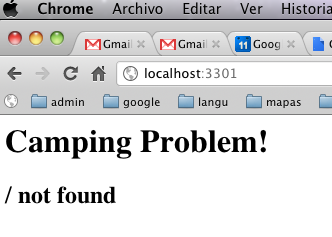
\includegraphics[scale=0.5]{chapter8/camping1.png}
\end{center}
\label{figure:camping1png}
\caption{Visitando la página (1)}
\end{figure}

Añadimos este código a \verb|nuts.rb|:
\begin{verbatim}
 module Nuts::Controllers
    class Index < R '/'
      def get
        Time.now.to_s
      end
    end
  end
\end{verbatim}

y lo ejecutamos de nuevo:
\begin{figure}[htb]
\begin{center}
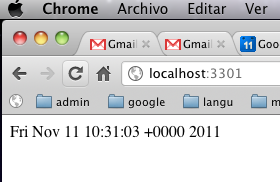
\includegraphics[scale=0.5]{chapter8/camping2.png}
\end{center}
\label{figure:camping2png}
\caption{Visitando la página (2)}
\end{figure}


